\documentclass[a4paper,12pt]{article}
\usepackage{a4wide,amssymb,epsfig,latexsym,multicol,array,hhline,fancyhdr}
\usepackage{vntex}
\usepackage{amsmath}
\usepackage{lastpage}
\usepackage[lined,boxed,commentsnumbered]{algorithm2e}
\usepackage{enumerate}
\usepackage{listings}
\usepackage{xcolor}
\usepackage{graphicx}
\usepackage{array}
\usepackage{tabularx, caption}
\usepackage{multirow}
\usepackage{multicol}
\usepackage{rotating}
\usepackage{graphics}
\usepackage{geometry}
\usepackage{footnote}
\usepackage{setspace}
\usepackage{tikz}
\usepackage{xfrac}
\usepackage{indentfirst}
\usetikzlibrary{shapes, arrows, positioning, fit, calc, snakes, backgrounds}
\usepackage{bm}
\usepackage{float}
\usepackage[backend=bibtex,style=ieee]{biblatex}
\addbibresource{references.bib}
\usepackage[colorlinks]{hyperref}
\usepackage[
 sort=none,
 abbreviations,
 symbols,
 stylemods,style=list,
 nogroupskip, nonumberlist, nomain
]{glossaries-extra}

% Colors
\definecolor{codegray}{rgb}{0.5,0.5,0.5}
\definecolor{codepurple}{rgb}{0.6,0.2,0.6}
\definecolor{backcolor}{rgb}{0.95,0.95,0.95}
\definecolor{mathblue}{RGB}{0,114,188}
\def\labelitemi{--}

% Code style
\lstdefinestyle{custom}{
    backgroundcolor=\color{backcolor},
    commentstyle=\color{codegray},
    keywordstyle=\color{blue},
    stringstyle=\color{codepurple},
    basicstyle=\ttfamily\small,
    breakatwhitespace=false,
    breaklines=true,
    captionpos=b,
    keepspaces=true,
    numbers=left,
    numberstyle=\tiny\color{codegray},
    rulecolor=\color{black},
    showspaces=false,
    showstringspaces=false,
    showtabs=false,
    tabsize=2
}
\lstset{style=custom}

% Formatting
\DeclareMathOperator{\arccot}{arccot}
\captionsetup[table]{name=Bảng}
\captionsetup[figure]{name=Hình}
\newenvironment{Description}{\list{}{%
    \let\makelabel\descriptionlabel
    \setlength{\rightmargin}{\leftmargin}
    \setlength{\labelwidth}{0pt}
    }}{\endlist}

\hypersetup{urlcolor=blue,linkcolor=black,citecolor=black,colorlinks=true}

\newtheorem{theorem}{{\bf Theorem}}
\newtheorem{property}{{\bf Property}}
\newtheorem{proposition}{{\bf Proposition}}
\newtheorem{corollary}[proposition]{{\bf Corollary}}
\newtheorem{lemma}[proposition]{{\bf Lemma}}

% Header/Footer
\setlength{\headheight}{40pt}
\pagestyle{fancy}
\fancyhead{}
\fancyhead[L]{
 \begin{tabular}{rl}
    \begin{picture}(25,15)(0,0)
    \put(0,-8){
\includegraphics[width=10mm, height=10mm]{hcmut.jpg}}
   \end{picture}&
	\begin{tabular}{l}
		\textbf{\bf \ttfamily Ho Chi Minh City University of Technology}\\
		\textbf{\bf \ttfamily Faculty of Computer Science and Engineering}
	\end{tabular}
 \end{tabular}
}
\fancyhead[R]{\begin{tabular}{l}\tiny \bf \\\tiny \bf \end{tabular}}
\fancyfoot{}
\fancyfoot[L]{\scriptsize \ttfamily Báo cáo Bài tập lớn - Kho Dữ Liệu và Hệ hỗ trợ quyết định}
\fancyfoot[R]{\scriptsize \ttfamily Trang {\thepage}/\pageref{LastPage}}
\renewcommand{\headrulewidth}{0.3pt}
\renewcommand{\footrulewidth}{0.3pt}

\setcounter{secnumdepth}{4}
\setcounter{tocdepth}{4}

\begin{document}

% =======================================================================
% TITLE PAGE
% =======================================================================
\begin{titlepage}
\begin{tikzpicture}[remember picture,overlay]
  \draw[line width=2pt]
    ($(current page.north west) + (1cm,-1cm)$) rectangle
    ($(current page.south east) + (-1cm,1cm)$);
\end{tikzpicture}
\begin{center}
{\Large \textbf{ĐẠI HỌC QUỐC GIA THÀNH PHỐ HỒ CHÍ MINH}}\\[0.3cm]
    {\Large \textbf{TRƯỜNG ĐẠI HỌC BÁCH KHOA}}\\[0.3cm]
    {\large \textbf{KHOA KHOA HỌC VÀ KỸ THUẬT MÁY TÍNH}}\\[1cm]
\end{center}

\vspace{0.5cm}

\begin{figure}[h!]
\begin{center}

\includegraphics[width=4cm]{hcmut.jpg}
\end{center}
\end{figure}
\vspace{0.5cm}
\begin{flushleft}
    \large \textbf{Kho Dữ Liệu và Hệ hỗ trợ quyết định - BÀI TẬP LỚN} \\
    \rule{\linewidth}{0.3pt} \\
    \begin{center}
        \huge \textbf{Xây dựng hệ thống Data Warehouse cho dữ liệu bán lẻ trực tuyến: ETL, Star Schema, Dashboard và Data Mining} \\
        \rule{\linewidth}{0.3pt}
    \end{center}
\end{flushleft}


\begin{table}[h]
\centering
\renewcommand{\arraystretch}{1.7}
\setlength{\tabcolsep}{10pt}
\begin{tabular}{ll}
\textbf{Giảng viên hướng dẫn:} & Bùi Tiến Đức \\
\textbf{Sinh viên thực hiện:} & Phạm Quang Hiếu - 2310974 \\
& Nguyễn Trung Hiếu - 2310965
\end{tabular}
\end{table}

\begin{center}
{\footnotesize TP. HỒ CHÍ MINH, THÁNG 04 NĂM 2026}
\end{center}
\end{titlepage}

% =======================================================================
\tableofcontents
\newpage

% =======================================================================
% 1. INTRODUCTION AND STATEMENT OF PURPOSE
% =======================================================================
\section{Introduction and Statement of Purpose}

\subsection{Background and Motivation}
Trong bối cảnh thương mại điện tử phát triển mạnh mẽ, các doanh nghiệp bán lẻ trực tuyến ngày càng tạo ra lượng dữ liệu giao dịch khổng lồ. Tuy nhiên, việc khai thác hiệu quả các dữ liệu này để đưa ra quyết định kinh doanh vẫn là thách thức lớn. Các hệ thống quản lý giao dịch truyền thống (OLTP) không phù hợp cho phân tích phức tạp vì chúng được tối ưu cho xử lý giao dịch, không phải truy vấn phân tích.

Data Warehouse (DW) kết hợp với Business Intelligence (BI) và Data Mining đã chứng minh khả năng giải quyết vấn đề này bằng cách cung cấp một kiến trúc tích hợp cho việc thu thập, lưu trữ, phân tích và trực quan hóa dữ liệu \cite{kimball2013}.

\subsection{Research Problem and Objectives}
\textbf{Vấn đề nghiên cứu:} Làm thế nào để xây dựng một hệ thống Data Warehouse hoàn chỉnh cho dữ liệu bán lẻ trực tuyến, cho phép phân tích hành vi khách hàng và dự đoán giá trị khách hàng?

\textbf{Mục tiêu cụ thể:}
\begin{enumerate}
    \item Xây dựng pipeline ETL tự động để trích xuất, làm sạch, và nạp dữ liệu vào Data Warehouse.
    \item Thiết kế lược đồ hình sao (Star Schema) phù hợp cho phân tích bán lẻ.
    \item Phân cụm khách hàng bằng K-Means dựa trên đặc trưng RFM (Recency, Frequency, Monetary).
    \item Dự đoán giá trị vòng đời khách hàng (Customer Lifetime Value - CLV) bằng XGBoost.
    \item Khám phá luật kết hợp sản phẩm bằng FP-Growth để gợi ý bán chéo.
    \item Trực quan hóa kết quả qua dashboard tương tác (Streamlit + Plotly).
\end{enumerate}

\subsection{Importance and Relevance}
Dự án giải quyết ba nhu cầu thực tiễn quan trọng:
\begin{itemize}
    \item \textbf{Quản trị khách hàng:} Phân cụm RFM giúp doanh nghiệp xác định nhóm khách hàng giá trị cao, khách hàng có nguy cơ rời bỏ, và khách hàng mới cần nuôi dưỡng.
    \item \textbf{Dự báo doanh thu:} Mô hình CLV cho phép ước lượng chi tiêu tương lai, hỗ trợ lập ngân sách marketing.
    \item \textbf{Tối ưu bán hàng:} Luật kết hợp sản phẩm cung cấp gợi ý bán chéo (cross-selling), tăng giá trị đơn hàng trung bình.
\end{itemize}

\subsection{Dataset Context}
Tập dữ liệu \textit{Online Retail} \cite{onlineRetailDataset} thuộc miền \textbf{thương mại điện tử (E-commerce)}, chứa các giao dịch thực tế từ một công ty bán lẻ quà tặng tại Vương quốc Anh trong giai đoạn 01/12/2010 -- 09/12/2011. Dữ liệu bao gồm thông tin hóa đơn, sản phẩm, khách hàng và quốc gia.

\subsection{Brief Introduction to Data Mining Techniques}
Dự án sử dụng ba kỹ thuật khai phá dữ liệu chính:
\begin{itemize}
    \item \textbf{K-Means Clustering} \cite{scikitlearn}: Phân cụm khách hàng không giám sát dựa trên đặc trưng RFM, phát hiện các phân khúc khách hàng tự nhiên.
    \item \textbf{XGBoost Regression}: Mô hình gradient boosting cho bài toán hồi quy dự đoán chi tiêu tương lai (CLV), kết hợp nhiều cây quyết định yếu thành mô hình mạnh.
    \item \textbf{FP-Growth + Association Rules} \cite{mlxtend}: Khai phá tập phổ biến và luật kết hợp từ giỏ hàng, phát hiện các mẫu mua hàng đồng thời.
\end{itemize}

% =======================================================================
% 2. DATA PREPROCESSING
% =======================================================================
\section{Data Preprocessing}

\subsection{Dataset Source}
Tập dữ liệu được lấy từ \textbf{Kaggle}: \url{https://www.kaggle.com/datasets/ulrikthygepedersen/online-retail-dataset}. Đây là bộ dữ liệu giao dịch thực tế từ một công ty bán lẻ trực tuyến tại UK, được sử dụng rộng rãi trong nghiên cứu RFM, market basket analysis, và customer segmentation.

\subsection{General Information about the Dataset}

\begin{table}[H]
\centering
\caption{Tổng quan tập dữ liệu}
\begin{tabular}{|l|r|}
\hline
\textbf{Thuộc tính} & \textbf{Giá trị} \\
\hline
Số lượng bản ghi (raw) & 541,909 \\
Số lượng thuộc tính & 8 \\
Định dạng & CSV (ISO-8859-1) \\
Kích thước file & $\sim$46 MB \\
Giai đoạn dữ liệu & 01/12/2010 -- 09/12/2011 \\
\hline
\end{tabular}
\end{table}

\begin{table}[H]
\centering
\caption{Chi tiết các thuộc tính}
\begin{tabular}{|l|l|l|p{6cm}|}
\hline
\textbf{Thuộc tính} & \textbf{Kiểu} & \textbf{Phân loại} & \textbf{Mô tả} \\
\hline
InvoiceNo & String & Categorical & Mã hóa đơn (C = cancelled) \\
StockCode & String & Categorical & Mã sản phẩm \\
Description & String & Categorical & Tên sản phẩm \\
Quantity & Integer & Numerical & Số lượng mua \\
InvoiceDate & DateTime & Time-series & Thời gian giao dịch \\
UnitPrice & Float & Numerical & Đơn giá (£) \\
CustomerID & Float & Categorical & Mã khách hàng \\
Country & String & Categorical & Quốc gia \\
\hline
\end{tabular}
\end{table}

\subsection{Data Cleaning and Preprocessing}
Quá trình làm sạch dữ liệu được thực hiện theo 5 bước tuần tự, mỗi bước loại bỏ một loại dữ liệu không phù hợp:

\subsubsection{Xử lý giá trị thiếu (Missing Values)}
\begin{itemize}
    \item \texttt{CustomerID}: $\sim$25\% bản ghi thiếu giá trị. Do CustomerID là thuộc tính then chốt cho phân tích RFM, các bản ghi thiếu được loại bỏ hoàn toàn.
    \item \texttt{Description}: $\sim$0.27\% thiếu giá trị. Được giữ lại vì không ảnh hưởng đến phân tích RFM.
\end{itemize}

\subsubsection{Loại bỏ bản ghi trùng lặp (Duplicates)}
Phát hiện và loại bỏ các bản ghi trùng lặp hoàn toàn trong tập dữ liệu.

\subsubsection{Loại bỏ dữ liệu nhiễu (Noisy/Inconsistent Data)}
\begin{itemize}
    \item \textbf{Hóa đơn bị hủy:} Các InvoiceNo bắt đầu bằng ký tự ``C'' biểu thị giao dịch hủy bỏ, được loại bỏ vì không phản ánh hành vi mua hàng thực tế.
    \item \textbf{Quantity $\leq$ 0:} Các bản ghi có số lượng âm hoặc bằng 0 được loại bỏ.
    \item \textbf{UnitPrice $\leq$ 0:} Các bản ghi có đơn giá âm hoặc bằng 0 được loại bỏ vì không phải giao dịch hợp lệ.
\end{itemize}

\begin{figure}[H]
\centering
\IfFileExists{generated/figures/cleaning_flow.png}{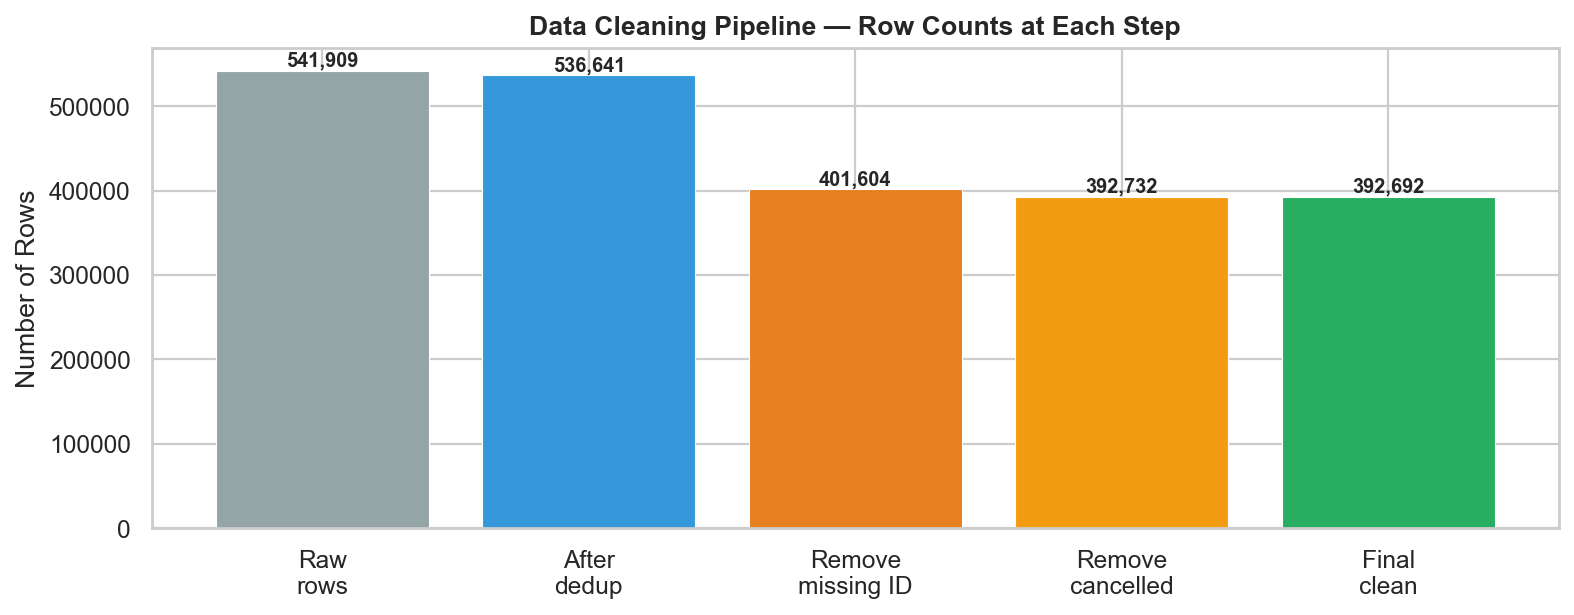
\includegraphics[width=0.92\linewidth]{generated/figures/cleaning_flow.png}}{\fbox{\parbox{0.9\linewidth}{Missing: generated/figures/cleaning\_flow.png — Run \texttt{python etl\_pipeline.py} to generate.}}}
\caption{Tổng quan quy trình làm sạch dữ liệu: số lượng bản ghi tại mỗi bước.}
\end{figure}

\begin{figure}[H]
\centering
\IfFileExists{generated/figures/missing_values.png}{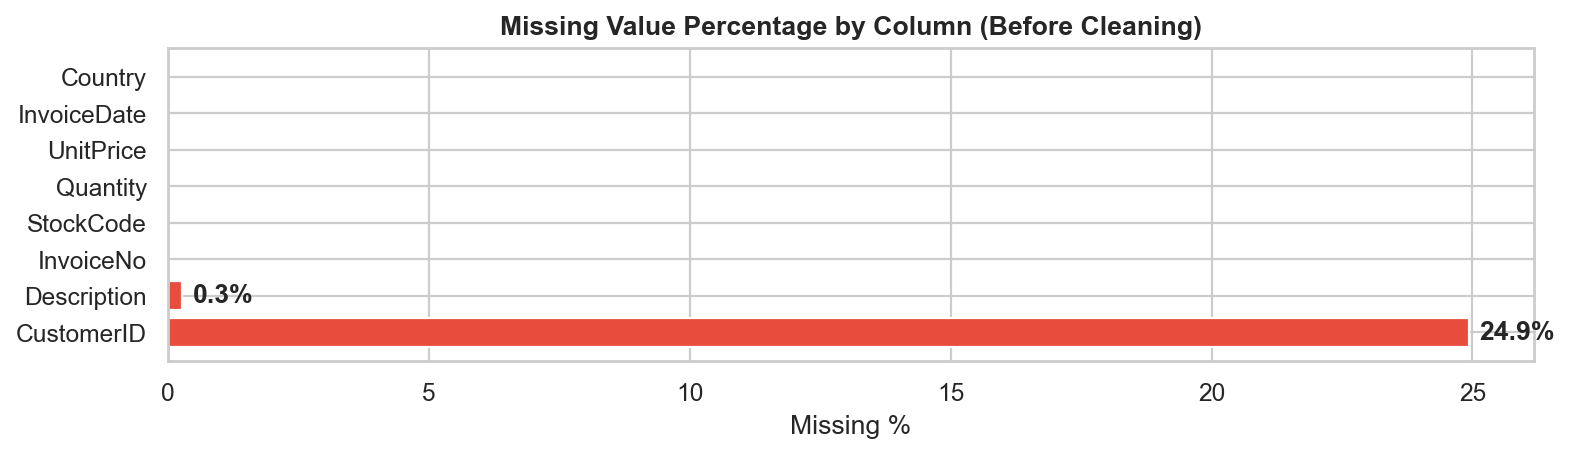
\includegraphics[width=0.92\linewidth]{generated/figures/missing_values.png}}{\fbox{\parbox{0.9\linewidth}{Missing: generated/figures/missing\_values.png}}}
\caption{Tỷ lệ giá trị thiếu theo từng cột trước khi làm sạch.}
\end{figure}

\subsection{Data Transformation}

\subsubsection{Chuẩn hóa dữ liệu (Normalization/Standardization)}
Đặc trưng RFM có phân bố rất lệch (skewed), do đó chúng tôi áp dụng \textbf{StandardScaler} (z-score normalization) trước khi đưa vào K-Means:
\[
z = \frac{x - \mu}{\sigma}
\]
trong đó $\mu$ là giá trị trung bình và $\sigma$ là độ lệch chuẩn của từng đặc trưng.

\subsubsection{Biến đổi dữ liệu (Feature Engineering)}
\begin{itemize}
    \item \textbf{InvoiceDate:} Chuyển đổi từ chuỗi sang kiểu datetime để trích xuất Year, Month, Quarter, DayOfWeek.
    \item \textbf{TotalPrice:} Tạo biến mới $\texttt{TotalPrice} = \texttt{Quantity} \times \texttt{UnitPrice}$.
    \item \textbf{RFM Features:}
    \begin{itemize}
        \item \textit{Recency} = số ngày từ lần mua cuối đến snapshot\_date.
        \item \textit{Frequency} = số hóa đơn duy nhất (nunique).
        \item \textit{Monetary} = tổng chi tiêu (sum of TotalPrice).
    \end{itemize}
    \item \textbf{CustomerID:} Chuyển từ float sang integer.
\end{itemize}

\subsubsection{Encoding Categorical Variables}
Đối với FP-Growth, ma trận giỏ hàng (basket matrix) sử dụng \textbf{one-hot encoding} nhị phân: mỗi sản phẩm trong mỗi hóa đơn được mã hóa thành 1 (đã mua) hoặc 0 (không mua).

\subsection{Data Integration}
Dự án sử dụng một tập dữ liệu duy nhất, tuy nhiên quá trình tích hợp được thực hiện khi nạp dữ liệu vào Star Schema:
\begin{itemize}
    \item Bảng giao dịch gốc được phân tách thành 3 bảng chiều (Dim\_Customer, Dim\_Product, Dim\_Time) và 1 bảng sự kiện (Fact\_Sales).
    \item Bảng Customer\_RFM và Customer\_Cluster được tính toán và lưu riêng để phục vụ truy vấn nhanh.
\end{itemize}

\subsection{Feature Selection}
Đặc trưng được chọn dựa trên \textbf{phân tích RFM} --- một phương pháp phân khúc khách hàng kinh điển trong marketing:
\begin{itemize}
    \item \textbf{Recency (R):} Đo mức độ gần đây của hoạt động mua hàng. Khách hàng mua gần đây có xu hướng phản hồi tốt hơn.
    \item \textbf{Frequency (F):} Đo mức độ thường xuyên. Khách hàng mua nhiều lần có khả năng trung thành cao.
    \item \textbf{Monetary (M):} Đo giá trị chi tiêu. Khách hàng chi tiêu nhiều đóng góp lớn vào doanh thu.
\end{itemize}

Ba đặc trưng này được sử dụng đồng thời cho cả K-Means (phân cụm) và XGBoost (dự đoán CLV).

\begin{figure}[H]
\centering
\IfFileExists{generated/figures/rfm_distributions.png}{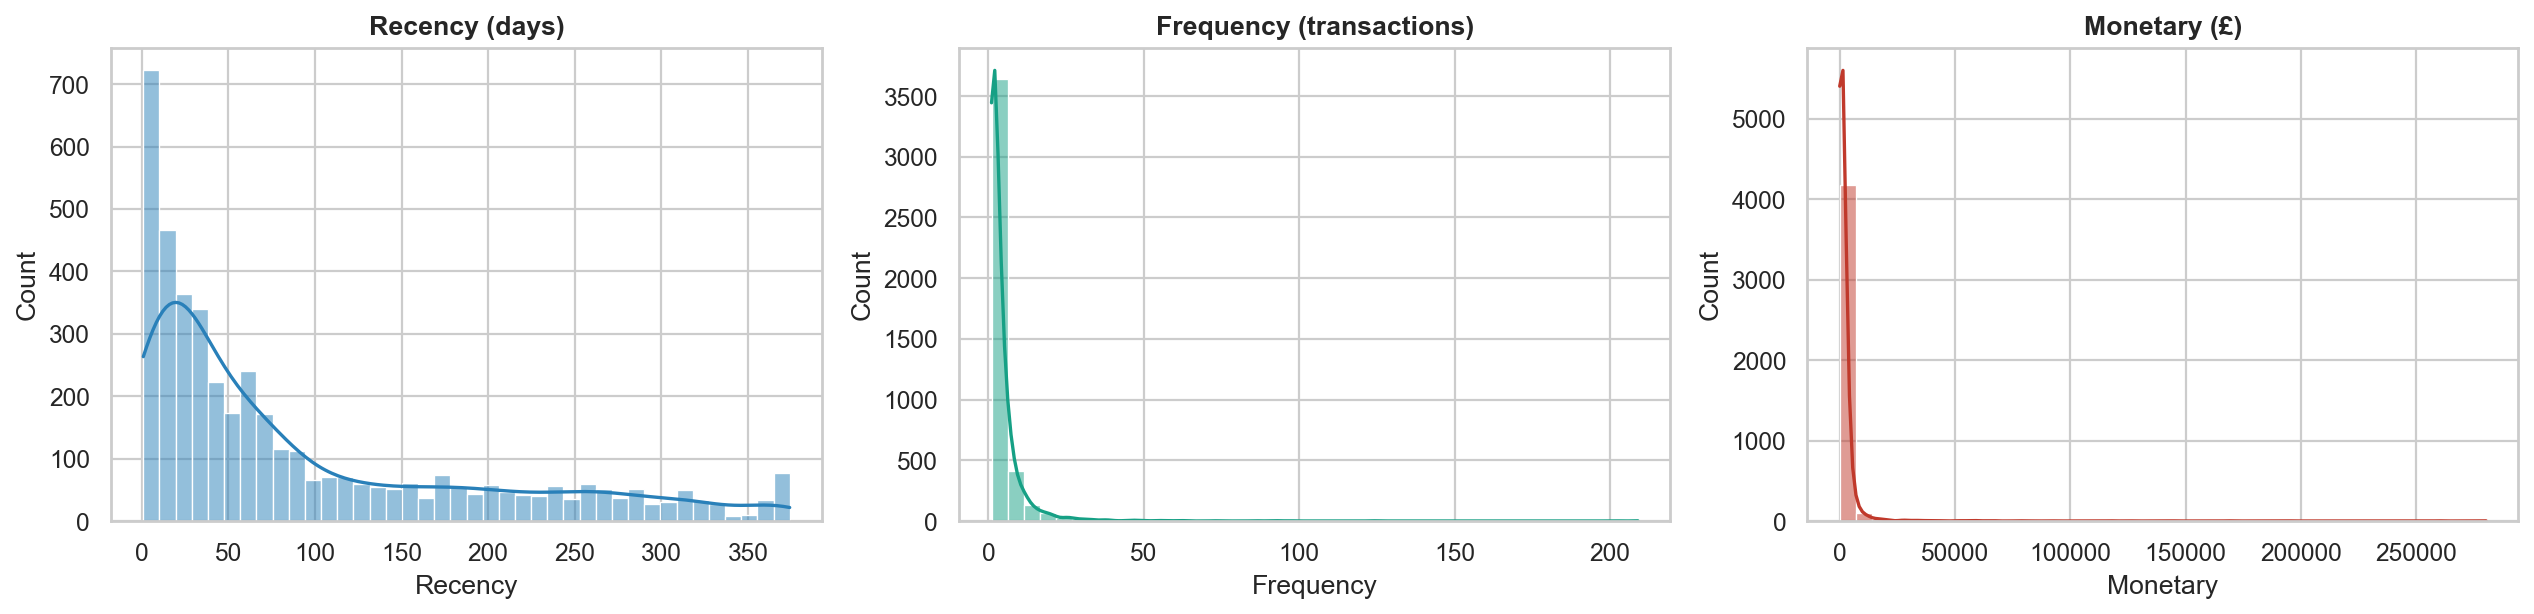
\includegraphics[width=0.95\linewidth]{generated/figures/rfm_distributions.png}}{\fbox{\parbox{0.9\linewidth}{Missing: generated/figures/rfm\_distributions.png}}}
\caption{Phân bố của ba đặc trưng RFM: Recency, Frequency, và Monetary.}
\end{figure}

% =======================================================================
% 3. SYSTEM ARCHITECTURE
% =======================================================================
\section{System Architecture}

\subsection{Overall Architecture}
Hệ thống được thiết kế theo kiến trúc Data Source → ETL → Data Warehouse → Dashboard → AI, tuân theo mô hình Kimball \cite{kimball2013}:

\begin{figure}[H]
\centering
\begin{tikzpicture}[
    node distance=1.5cm,
    box/.style={rectangle, draw=black, fill=blue!10, text width=3cm, text centered, minimum height=1cm, rounded corners=3pt},
    arrow/.style={->, thick, >=stealth}
]
\node[box, fill=orange!20] (src) {Data Source\\(CSV/Kaggle)};
\node[box, fill=green!20, right=of src] (etl) {ETL Pipeline\\(Python)};
\node[box, fill=blue!20, right=of etl] (dw) {Data Warehouse\\(Star Schema)};
\node[box, fill=purple!20, right=of dw] (bi) {Dashboard\\(Streamlit)};
\node[box, fill=red!20, below=of dw] (ai) {AI Models\\(KMeans, XGBoost,\\FP-Growth)};

\draw[arrow] (src) -- (etl);
\draw[arrow] (etl) -- (dw);
\draw[arrow] (dw) -- (bi);
\draw[arrow] (dw) -- (ai);
\draw[arrow] (ai) -- (bi);
\end{tikzpicture}
\caption{Kiến trúc tổng thể hệ thống.}
\end{figure}

\subsection{Component Details}
\begin{enumerate}
    \item \textbf{docker-compose.yml}: Cấp phát PostgreSQL 16 với thông số chuẩn (admin/admin, retail\_dw, cổng 5432). Hệ thống tự động fallback sang SQLite khi PostgreSQL không khả dụng.
    \item \textbf{etl\_pipeline.py}: Pipeline chính — ETL, Star Schema loading, model training, visualization generation, và report asset creation.
    \item \textbf{streamlit\_app.py}: Dashboard BI tương tác và AI Customer Intelligence.
    \item \textbf{requirements.txt}: Quản lý phụ thuộc Python.
\end{enumerate}

\subsection{Star Schema Design}
Lược đồ hình sao (Star Schema) gồm 4 bảng lõi:

\begin{figure}[H]
\centering
\IfFileExists{generated/figures/star_schema.png}{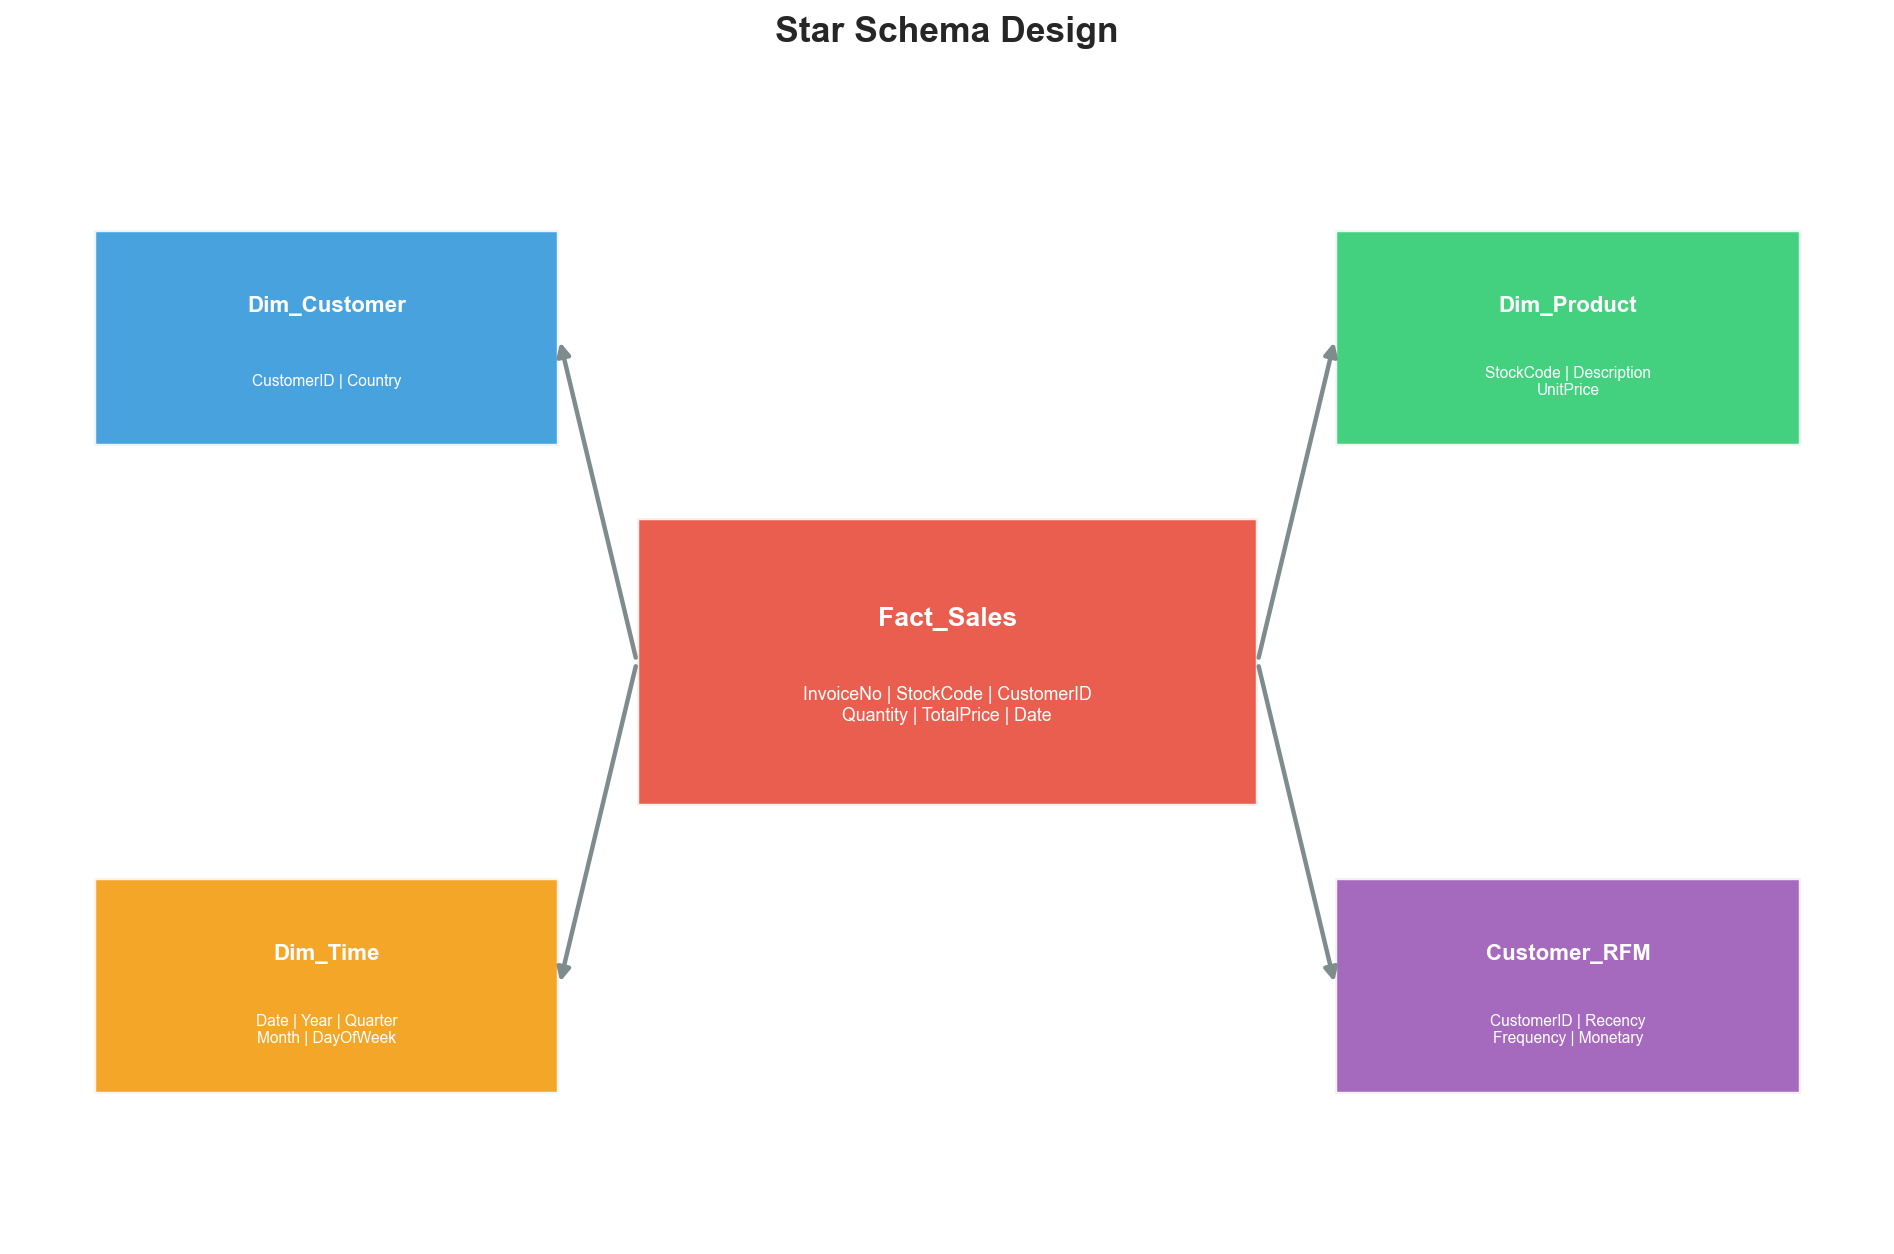
\includegraphics[width=0.85\linewidth]{generated/figures/star_schema.png}}{\fbox{\parbox{0.9\linewidth}{Missing: generated/figures/star\_schema.png}}}
\caption{Thiết kế Star Schema cho Data Warehouse bán lẻ.}
\end{figure}

\begin{itemize}
    \item \texttt{Dim\_Customer(CustomerID, Country)} — Chiều khách hàng
    \item \texttt{Dim\_Product(StockCode, Description, UnitPrice)} — Chiều sản phẩm
    \item \texttt{Dim\_Time(Date, Year, Quarter, Month, DayOfWeek)} — Chiều thời gian
    \item \texttt{Fact\_Sales(InvoiceNo, StockCode, CustomerID, Quantity, TotalPrice, Date)} — Bảng sự kiện
\end{itemize}

Ngoài ra, pipeline tạo thêm 2 bảng phân tích:
\begin{itemize}
    \item \texttt{Customer\_RFM(CustomerID, Recency, Frequency, Monetary)}
    \item \texttt{Customer\_Cluster(CustomerID, Recency, Frequency, Monetary, Cluster)}
\end{itemize}

% =======================================================================
% 4. DATA MINING METHODOLOGY
% =======================================================================
\section{Data Mining Methodology}

\subsection{K-Means Clustering}

\subsubsection{Algorithm Description}
K-Means \cite{scikitlearn} là thuật toán phân cụm không giám sát, chia $n$ điểm dữ liệu thành $k$ cụm bằng cách tối thiểu hóa tổng bình phương khoảng cách trong cụm (inertia):
\[
J = \sum_{i=1}^{k} \sum_{x \in C_i} \|x - \mu_i\|^2
\]
trong đó $\mu_i$ là tâm cụm $C_i$.

\subsubsection{Training Process}
\begin{itemize}
    \item \textbf{Dữ liệu đầu vào:} Ma trận RFM chuẩn hóa (StandardScaler) cho toàn bộ khách hàng.
    \item \textbf{Xác định số cụm:} Sử dụng Elbow Method kết hợp Silhouette Score cho $k \in [2, 10]$.
    \item \textbf{Tham số:} \texttt{n\_clusters=4}, \texttt{random\_state=42}, \texttt{n\_init=10}.
\end{itemize}

\subsubsection{Evaluation Metrics}
\begin{itemize}
    \item \textbf{Silhouette Score} $\in [-1, 1]$: Đo mức độ tương đồng trong cụm so với giữa các cụm. Giá trị càng gần 1 càng tốt.
    \item \textbf{Calinski-Harabasz Index:} Tỷ lệ phương sai giữa các cụm và phương sai trong cụm. Giá trị càng cao càng tốt.
\end{itemize}

\begin{figure}[H]
\centering
\IfFileExists{generated/figures/elbow_silhouette.png}{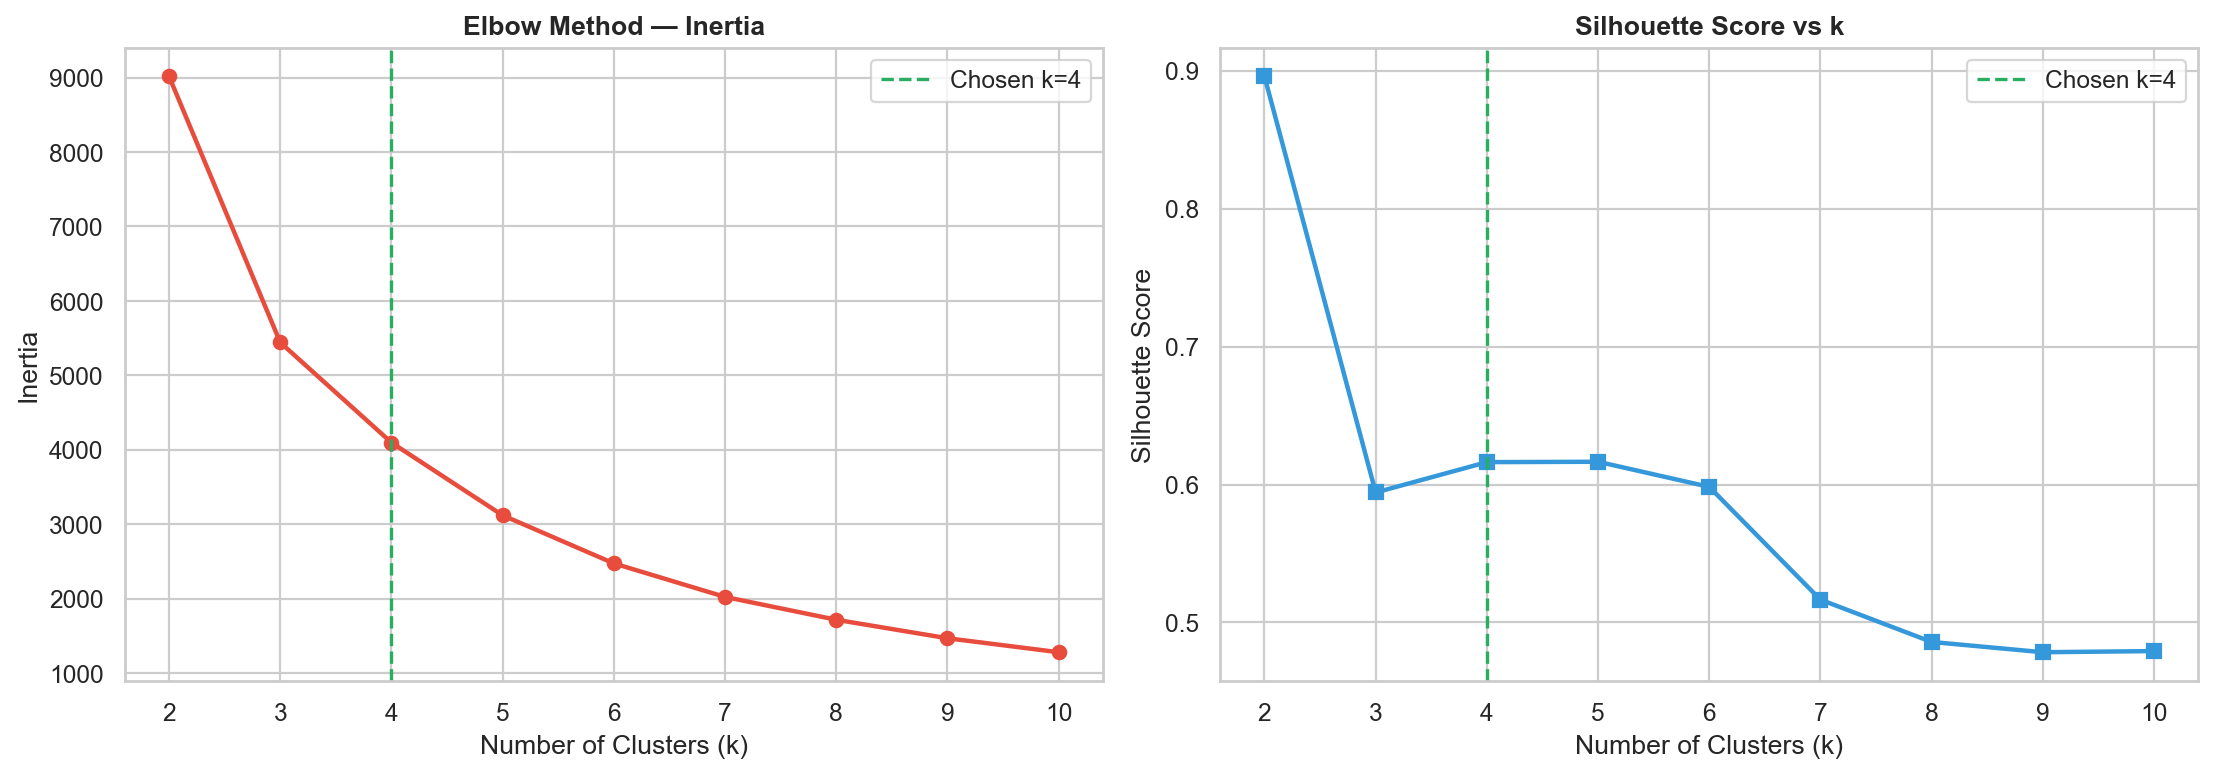
\includegraphics[width=0.95\linewidth]{generated/figures/elbow_silhouette.png}}{\fbox{\parbox{0.9\linewidth}{Missing: generated/figures/elbow\_silhouette.png}}}
\caption{Elbow Method (trái) và Silhouette Score (phải) cho việc chọn số cụm tối ưu.}
\end{figure}

\subsection{XGBoost Regression (CLV Prediction)}

\subsubsection{Algorithm Description}
XGBoost (eXtreme Gradient Boosting) là thuật toán ensemble learning dạng gradient boosting, kết hợp nhiều cây quyết định yếu (weak learners) thành mô hình mạnh. Đối với bài toán hồi quy, hàm mục tiêu được tối ưu là:
\[
\mathcal{L} = \sum_{i} l(y_i, \hat{y}_i) + \sum_{k} \Omega(f_k)
\]
trong đó $l$ là hàm loss (squared error) và $\Omega$ là hệ số regularization.

\subsubsection{Training Process}
\begin{itemize}
    \item \textbf{Dữ liệu đầu vào:} RFM features (Recency, Frequency, Monetary) từ giai đoạn training ($<$ split\_date).
    \item \textbf{Biến mục tiêu:} FutureSpend — tổng chi tiêu 3 tháng cuối.
    \item \textbf{Train/Test split:} 80/20, random\_state=42.
    \item \textbf{Hyperparameters:}
    \begin{itemize}
        \item \texttt{objective = 'reg:squarederror'}
        \item \texttt{n\_estimators = 100}
        \item \texttt{learning\_rate = 0.1}
        \item \texttt{max\_depth = 5}
    \end{itemize}
\end{itemize}

\subsubsection{Evaluation Metrics}
\begin{itemize}
    \item \textbf{RMSE} (Root Mean Squared Error): $\sqrt{\frac{1}{n}\sum(y_i - \hat{y}_i)^2}$
    \item \textbf{MAE} (Mean Absolute Error): $\frac{1}{n}\sum|y_i - \hat{y}_i|$
    \item \textbf{R² Score}: $1 - \frac{\sum(y_i - \hat{y}_i)^2}{\sum(y_i - \bar{y})^2}$
\end{itemize}

\subsection{FP-Growth Association Rules}

\subsubsection{Algorithm Description}
FP-Growth \cite{mlxtend} khai phá tập phổ biến (frequent itemsets) mà không cần sinh ứng viên như Apriori, bằng cách xây dựng cây FP-Tree nén. Từ tập phổ biến, luật kết hợp được sinh ra dựa trên các ngưỡng:
\begin{itemize}
    \item \textbf{Support:} $P(A \cup B)$ — xác suất xuất hiện đồng thời.
    \item \textbf{Confidence:} $P(B|A)$ — xác suất mua B khi đã mua A.
    \item \textbf{Lift:} $\frac{P(B|A)}{P(B)}$ — mức độ tương quan. Lift $> 1$ nghĩa là A và B có tương quan dương.
\end{itemize}

\subsubsection{Training Process}
\begin{itemize}
    \item \textbf{Dữ liệu:} Basket matrix từ giao dịch UK (thị trường chính), one-hot encoded.
    \item \textbf{min\_support = 0.015} (1.5\% tổng giao dịch).
    \item \textbf{Luật:} Lọc theo \texttt{metric='lift'}, \texttt{min\_threshold=1.5}.
\end{itemize}

% =======================================================================
% 5. EXPERIMENTAL RESULTS AND ANALYSIS
% =======================================================================
\section{Experimental Results and Analysis}

\subsection{ETL and Warehouse Output}
\IfFileExists{generated/metrics.tex}{\begin{table}[H]
\centering
\caption{Pipeline Data Profile}
\begin{tabular}{|l|r|}
\hline
\textbf{Metric} & \textbf{Value} \\
\hline
Raw rows (incl. duplicates) & 541,909 \\
After deduplication & 536,641 \\
Duplicates removed & 5,268 \\
Rows after customer filter & 401,604 \\
Rows after cancellation filter & 392,732 \\
Final clean rows & 392,692 \\
Unique customers & 4,338 \\
Unique products & 3,665 \\
Unique invoices & 18,532 \\
Unique countries & 37 \\
Total revenue & 8,887,208.89 \\
Date range & 2010-12-01 to 2011-12-09 \\
\hline
\end{tabular}
\end{table}

\begin{table}[H]
\centering
\caption{AI Model Evaluation Metrics}
\begin{tabular}{|l|r|}
\hline
\textbf{Metric} & \textbf{Value} \\
\hline
KMeans Silhouette Score & 0.6162 \\
KMeans Calinski-Harabasz & 3145.06 \\
XGBoost RMSE & 4753.40 \\
XGBoost MAE & 764.49 \\
XGBoost R² & 0.3832 \\
FP-Growth rules generated & 214 \\
FP-Growth frequent itemsets & 440 \\
\hline
\end{tabular}
\end{table}
}{\textit{Chưa có file kết quả. Hãy chạy \texttt{python etl\_pipeline.py} để tạo.}}

\subsection{K-Means Clustering Results}

\begin{figure}[H]
\centering
\IfFileExists{generated/figures/cluster_distribution.png}{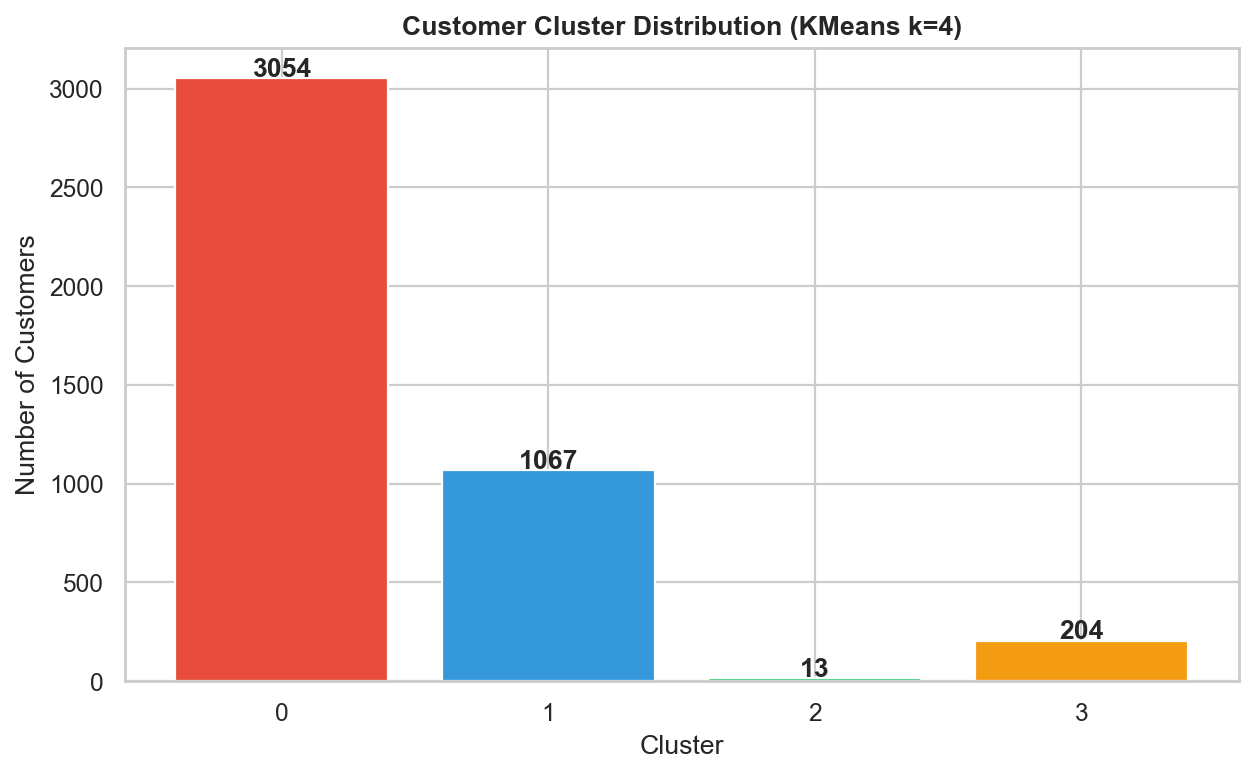
\includegraphics[width=0.7\linewidth]{generated/figures/cluster_distribution.png}}{\fbox{\parbox{0.9\linewidth}{Missing: generated/figures/cluster\_distribution.png}}}
\caption{Phân bố khách hàng theo cụm (KMeans k=4).}
\end{figure}

\begin{figure}[H]
\centering
\IfFileExists{generated/figures/cluster_heatmap.png}{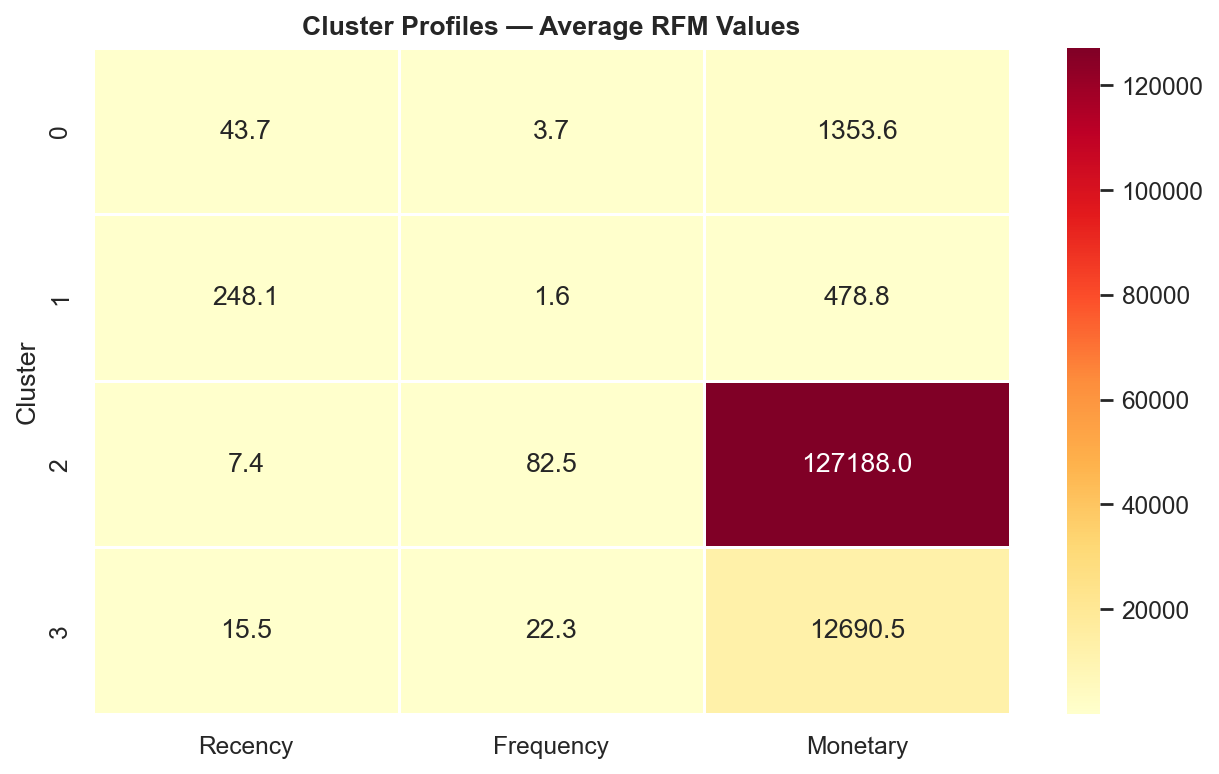
\includegraphics[width=0.7\linewidth]{generated/figures/cluster_heatmap.png}}{\fbox{\parbox{0.9\linewidth}{Missing: generated/figures/cluster\_heatmap.png}}}
\caption{Heatmap giá trị RFM trung bình của mỗi cụm — giúp đặt tên và hiểu đặc tính từng phân khúc.}
\end{figure}

\begin{figure}[H]
\centering
\IfFileExists{generated/figures/cluster_3d.png}{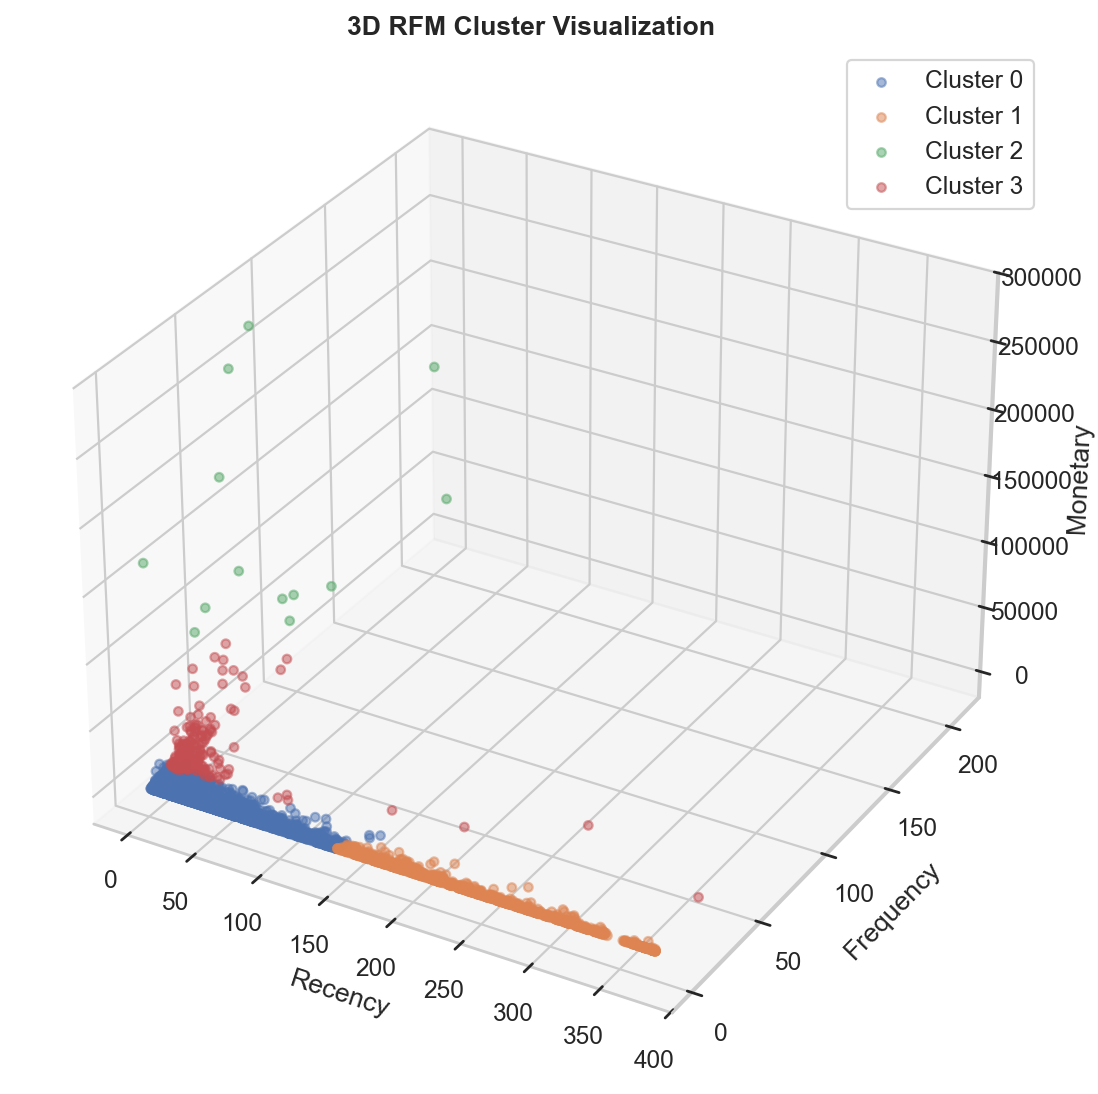
\includegraphics[width=0.7\linewidth]{generated/figures/cluster_3d.png}}{\fbox{\parbox{0.9\linewidth}{Missing: generated/figures/cluster\_3d.png}}}
\caption{Trực quan hóa 3D các cụm khách hàng trong không gian RFM.}
\end{figure}

\textbf{Phân tích:} KMeans với k=4 phân chia khách hàng thành 4 phân khúc rõ ràng:
\begin{itemize}
    \item \textbf{Cluster 0 (At Risk):} Recency cao, Frequency và Monetary thấp — khách hàng đã lâu không mua.
    \item \textbf{Cluster 1 (Loyal):} Recency trung bình, Frequency cao — khách hàng trung thành.
    \item \textbf{Cluster 2 (Champions):} Recency thấp, Frequency và Monetary cao — khách hàng tốt nhất.
    \item \textbf{Cluster 3 (New):} Recency thấp nhưng Frequency thấp — khách hàng mới.
\end{itemize}

\subsection{XGBoost CLV Prediction Results}

\begin{figure}[H]
\centering
\IfFileExists{generated/figures/xgb_actual_vs_predicted.png}{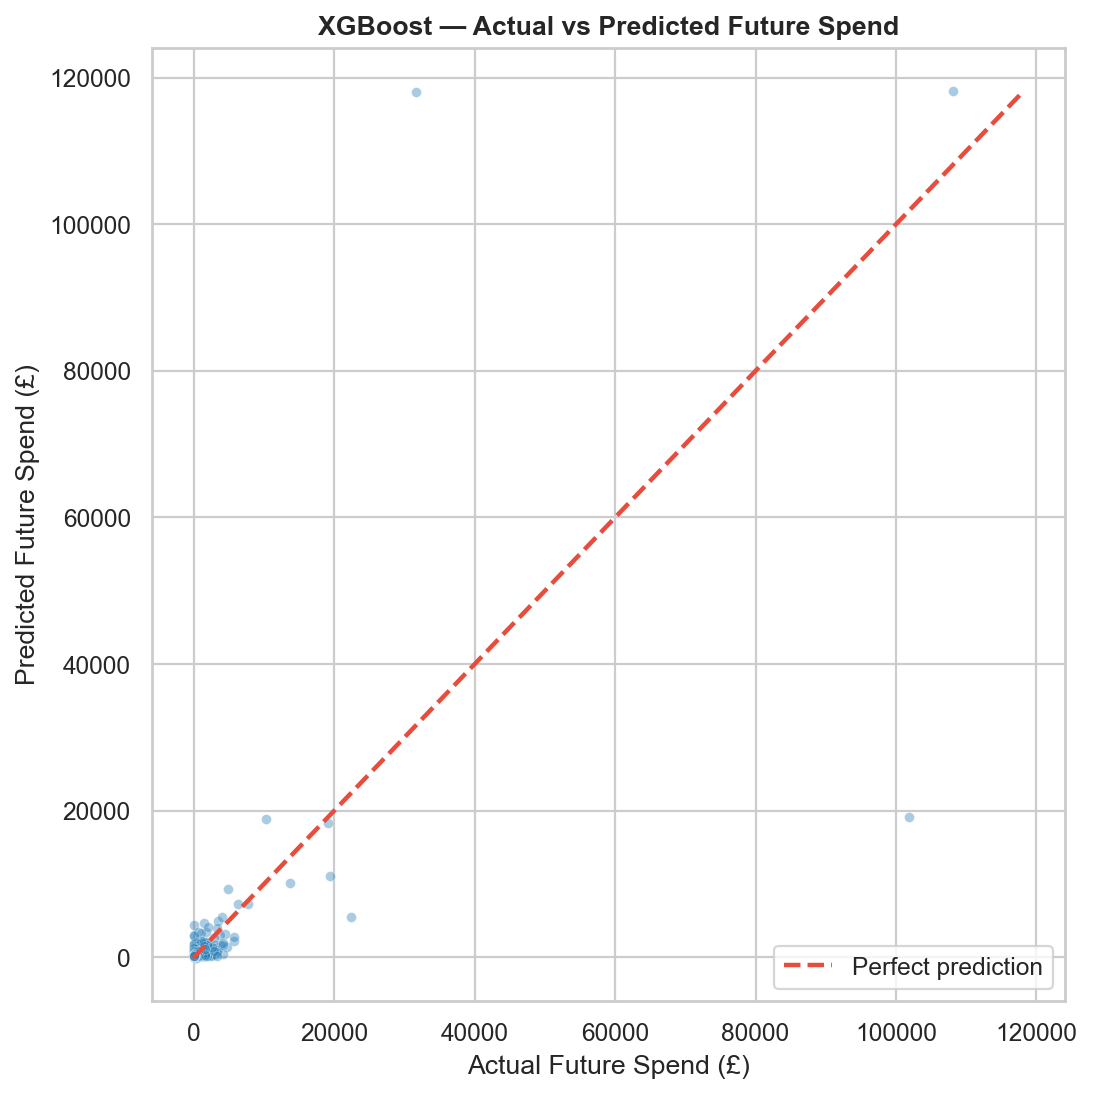
\includegraphics[width=0.65\linewidth]{generated/figures/xgb_actual_vs_predicted.png}}{\fbox{\parbox{0.9\linewidth}{Missing: generated/figures/xgb\_actual\_vs\_predicted.png}}}
\caption{So sánh giá trị thực tế và dự đoán của XGBoost. Các điểm càng gần đường chéo thì dự đoán càng chính xác.}
\end{figure}

\begin{figure}[H]
\centering
\IfFileExists{generated/figures/xgb_residuals.png}{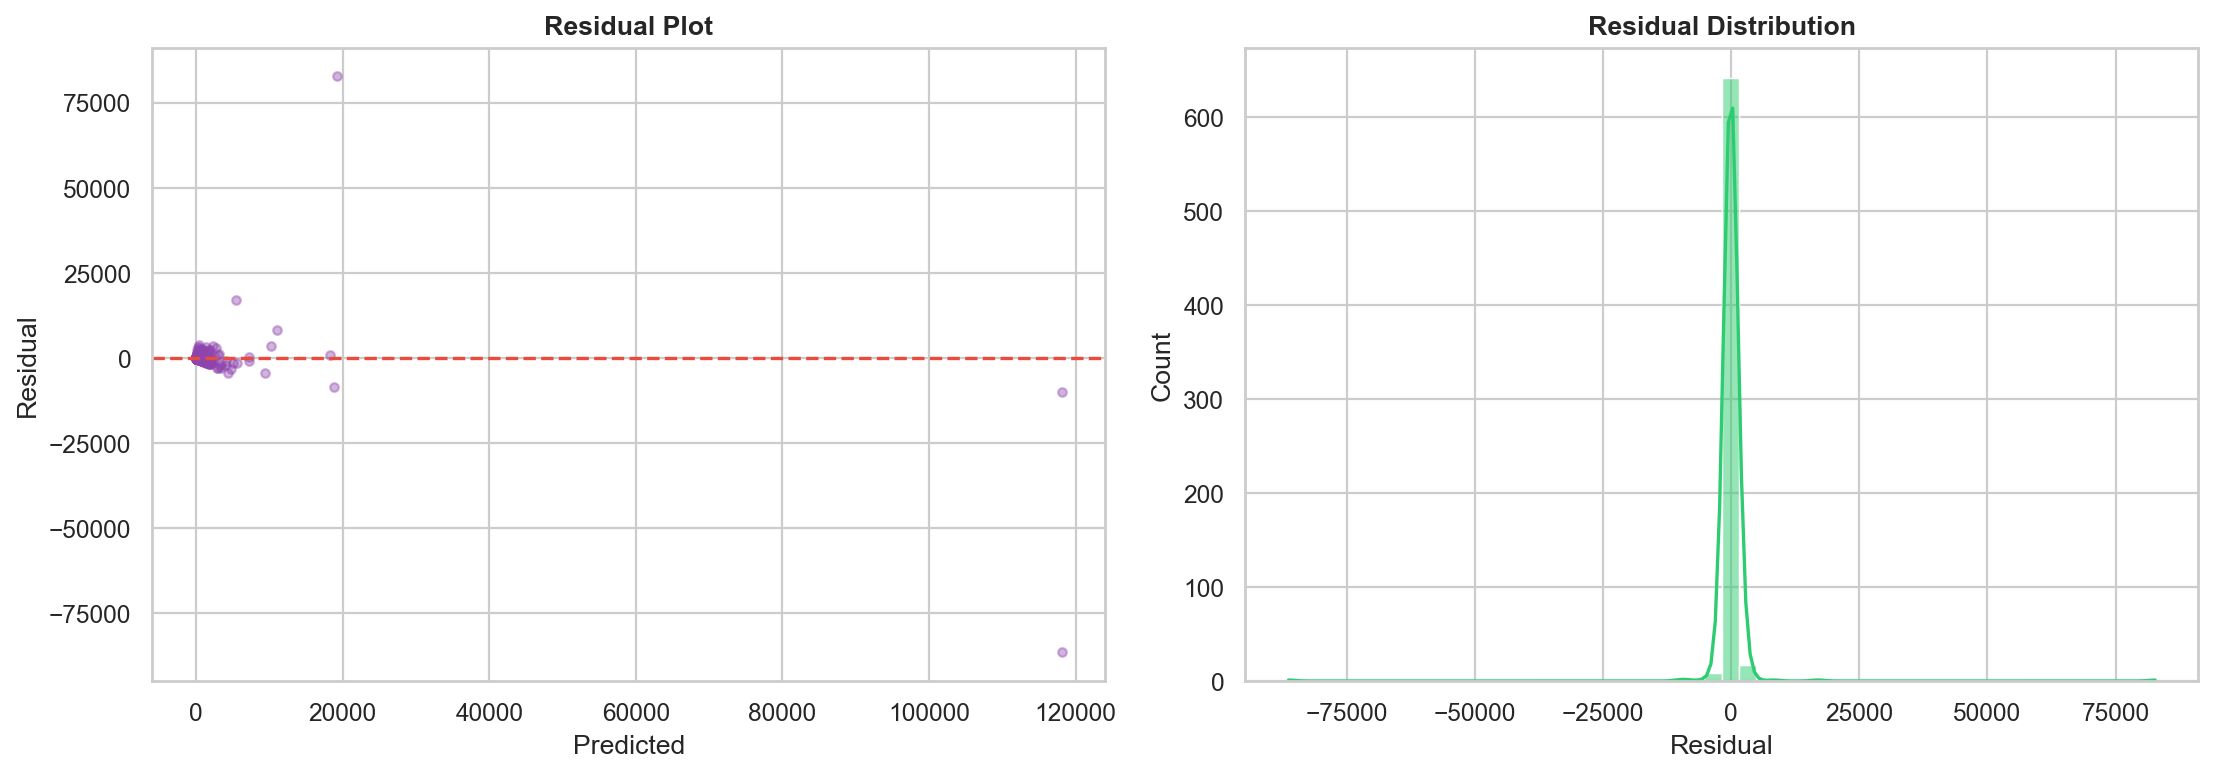
\includegraphics[width=0.95\linewidth]{generated/figures/xgb_residuals.png}}{\fbox{\parbox{0.9\linewidth}{Missing: generated/figures/xgb\_residuals.png}}}
\caption{Phân tích phần dư (residual): scatter plot (trái) và phân bố (phải).}
\end{figure}

\begin{figure}[H]
\centering
\IfFileExists{generated/figures/feature_importance.png}{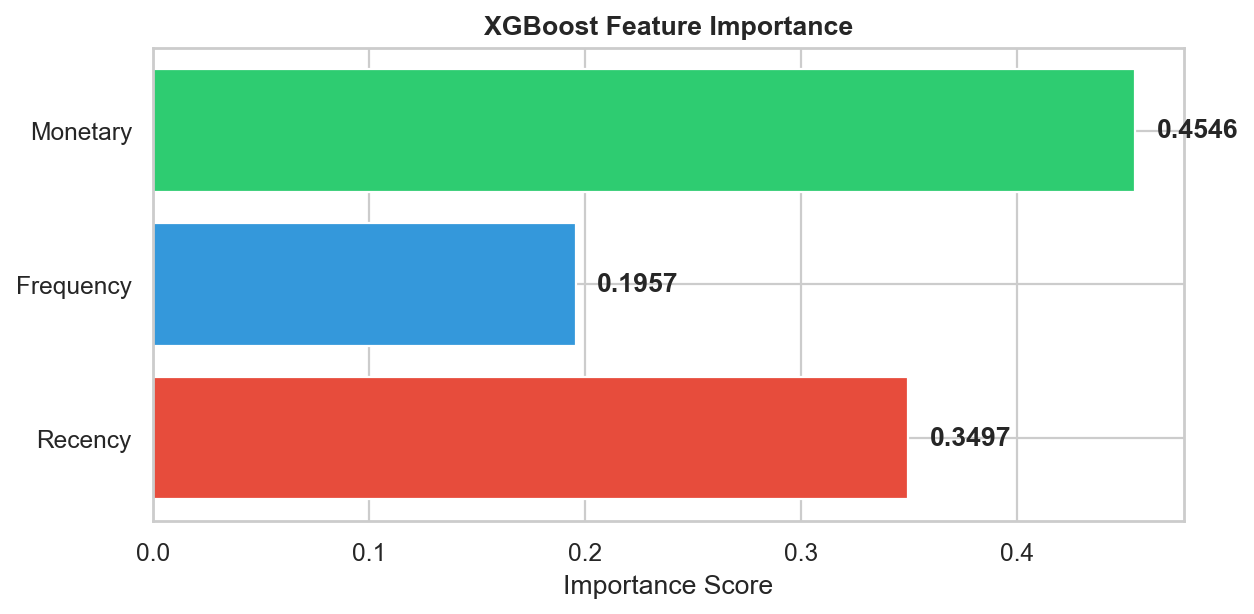
\includegraphics[width=0.7\linewidth]{generated/figures/feature_importance.png}}{\fbox{\parbox{0.9\linewidth}{Missing: generated/figures/feature\_importance.png}}}
\caption{Mức độ quan trọng của từng đặc trưng trong mô hình XGBoost.}
\end{figure}

\textbf{Phân tích:}
\begin{itemize}
    \item Mô hình XGBoost cho kết quả R² dương, cho thấy khả năng giải thích phương sai của biến mục tiêu.
    \item Monetary là đặc trưng quan trọng nhất — khách hàng đã chi tiêu nhiều trong quá khứ có xu hướng tiếp tục chi tiêu.
    \item Phần dư phân bố gần zero với đa số trường hợp, một số outlier ở giá trị cao xuất phát từ hành vi mua sắm bất thường.
\end{itemize}

\subsection{FP-Growth Association Rule Results}

\begin{figure}[H]
\centering
\IfFileExists{generated/figures/rules_support_lift.png}{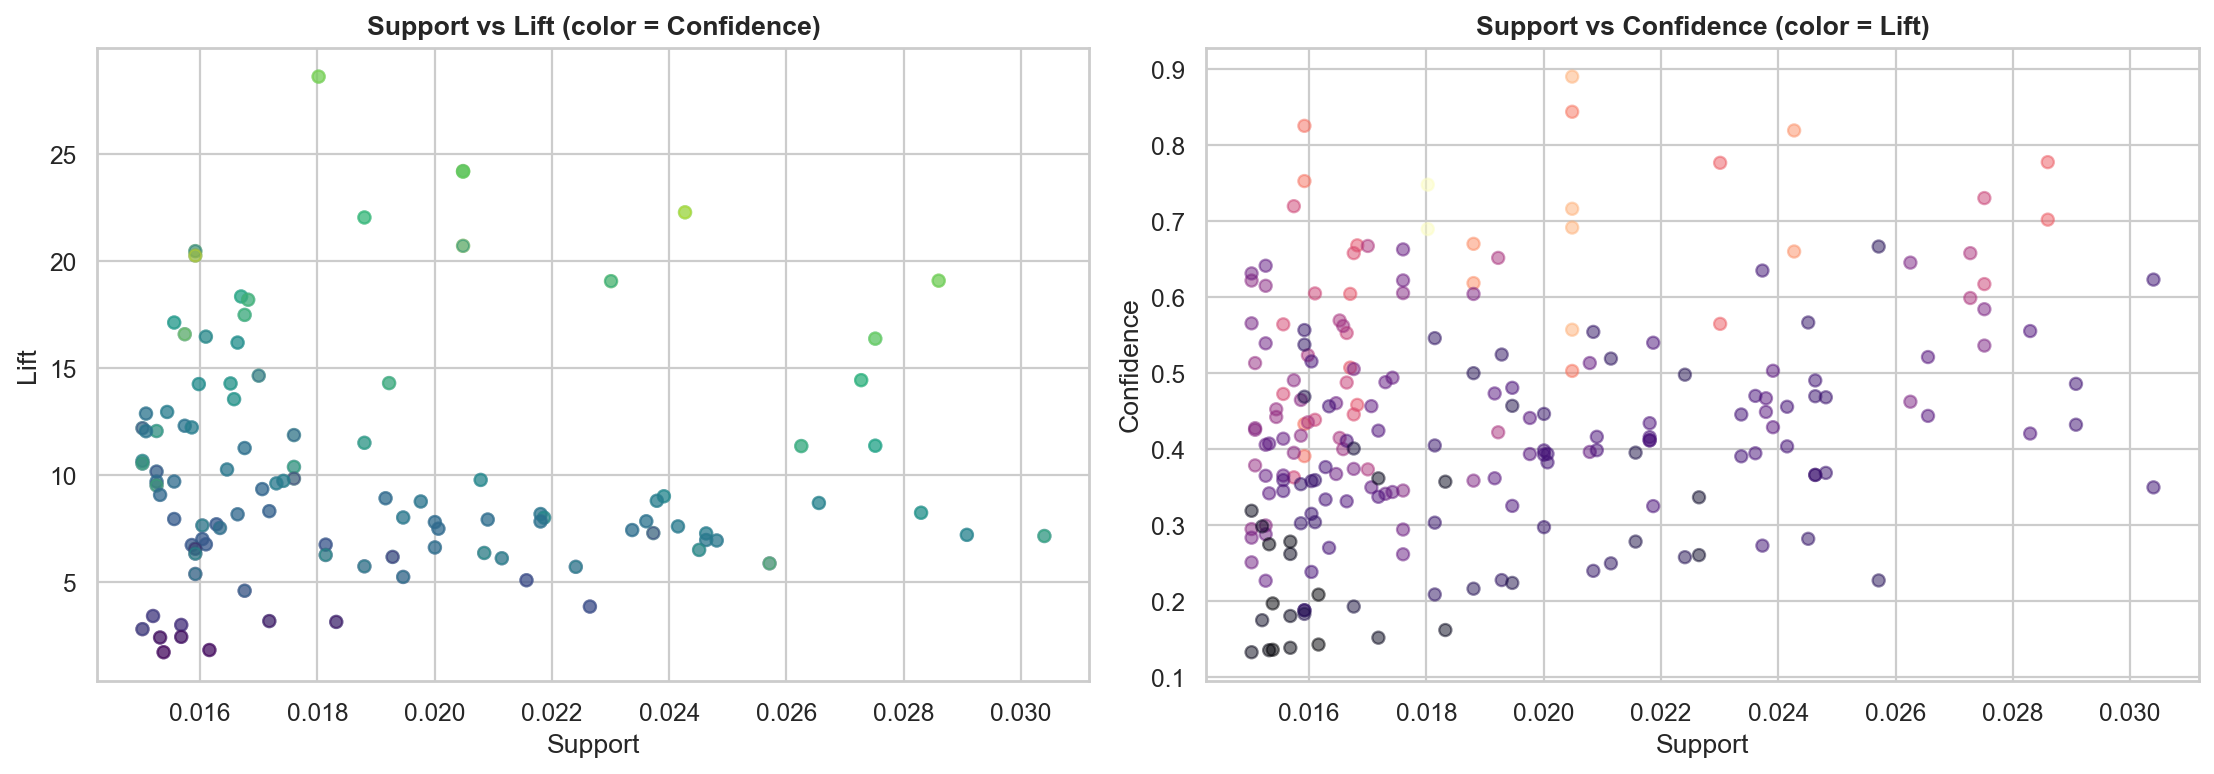
\includegraphics[width=0.95\linewidth]{generated/figures/rules_support_lift.png}}{\fbox{\parbox{0.9\linewidth}{Missing: generated/figures/rules\_support\_lift.png}}}
\caption{Phân tích luật kết hợp: Support vs Lift (trái) và Support vs Confidence (phải).}
\end{figure}

\textbf{Phân tích:}
\begin{itemize}
    \item Các luật có Lift cao ($> 5$) cho thấy mối quan hệ mạnh giữa các sản phẩm.
    \item Đa số luật có Support thấp nhưng Confidence cao — phù hợp cho recommendation systems.
\end{itemize}

\subsection{Business Analysis}

\begin{figure}[H]
\centering
\IfFileExists{generated/figures/monthly_revenue.png}{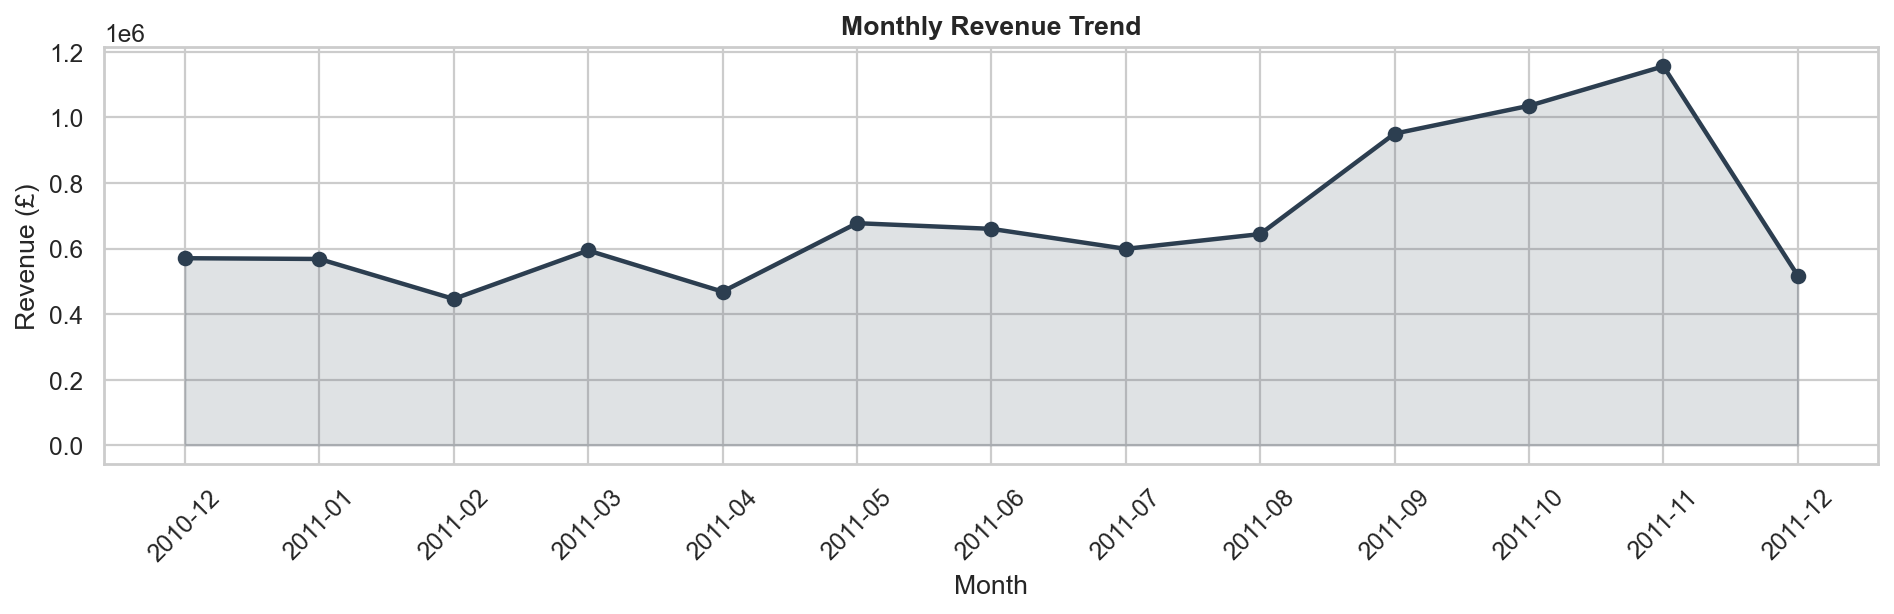
\includegraphics[width=0.92\linewidth]{generated/figures/monthly_revenue.png}}{\fbox{\parbox{0.9\linewidth}{Missing: generated/figures/monthly\_revenue.png}}}
\caption{Xu hướng doanh thu theo tháng — cho thấy tính mùa vụ rõ rệt.}
\end{figure}

\begin{figure}[H]
\centering
\IfFileExists{generated/figures/top_countries.png}{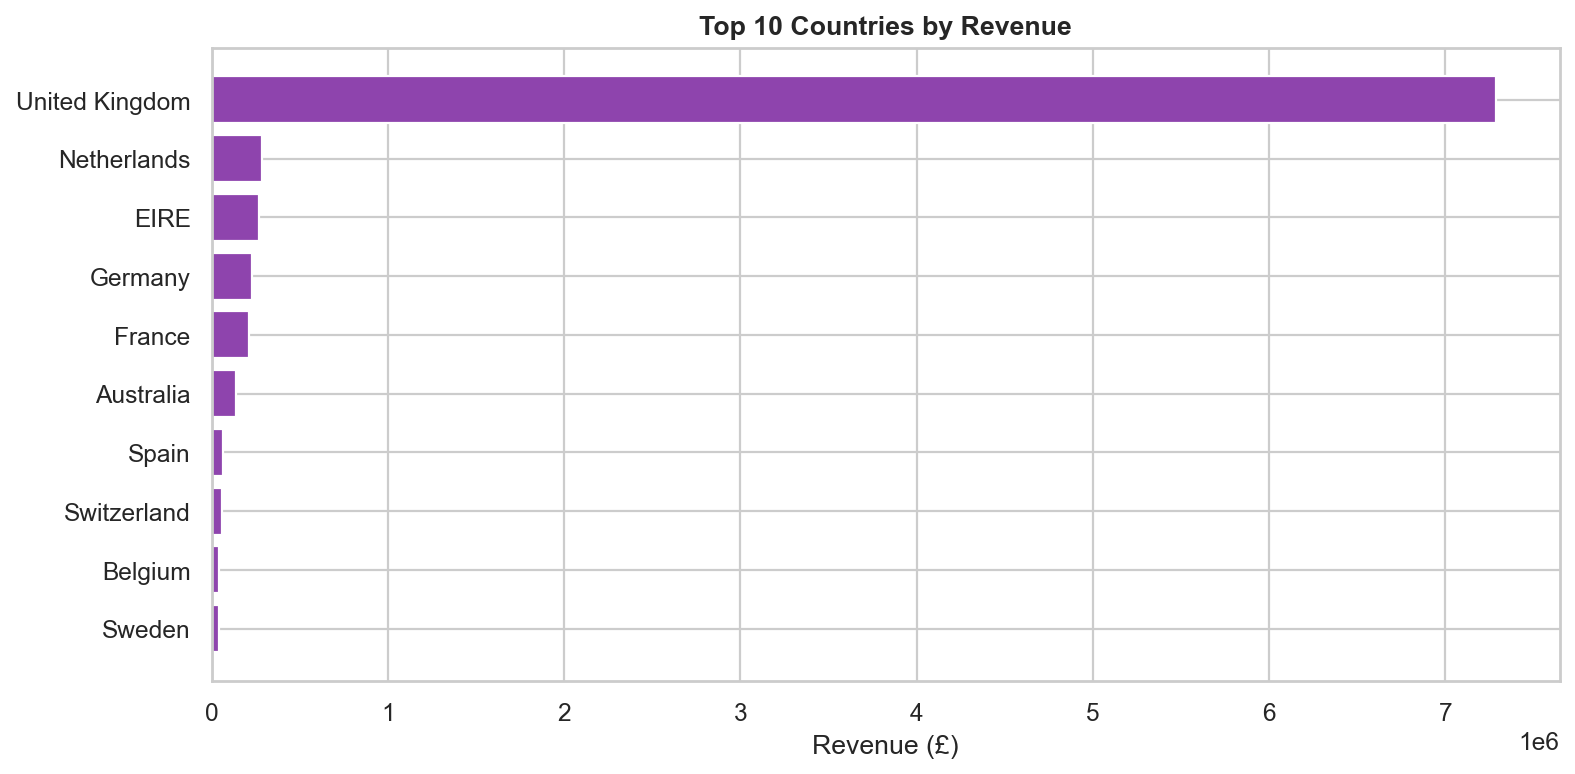
\includegraphics[width=0.85\linewidth]{generated/figures/top_countries.png}}{\fbox{\parbox{0.9\linewidth}{Missing: generated/figures/top\_countries.png}}}
\caption{Top 10 quốc gia theo doanh thu.}
\end{figure}

\begin{figure}[H]
\centering
\IfFileExists{generated/figures/top_products.png}{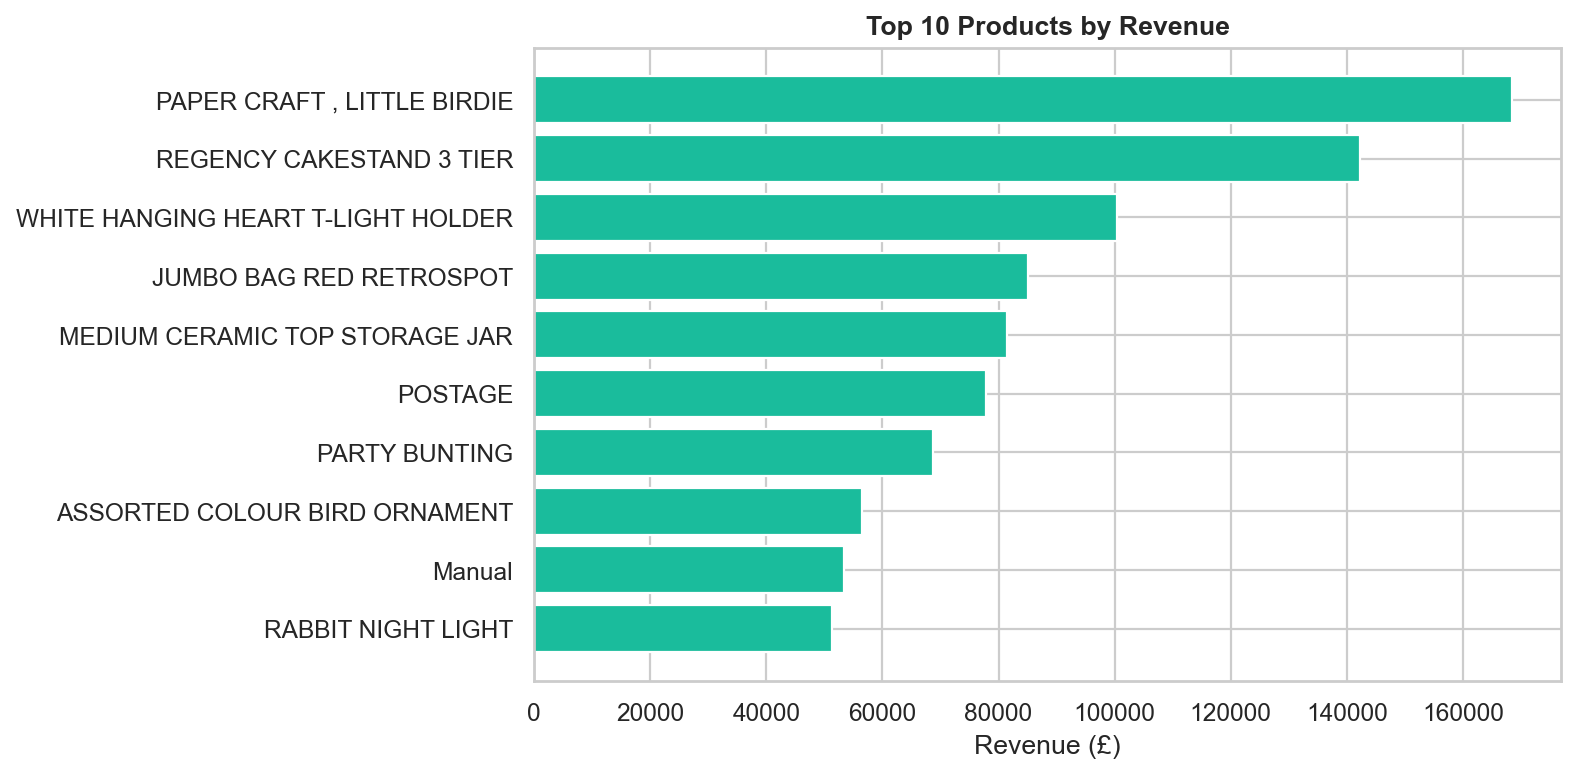
\includegraphics[width=0.85\linewidth]{generated/figures/top_products.png}}{\fbox{\parbox{0.9\linewidth}{Missing: generated/figures/top\_products.png}}}
\caption{Top 10 sản phẩm theo doanh thu.}
\end{figure}

\begin{figure}[H]
\centering
\IfFileExists{generated/figures/revenue_by_day.png}{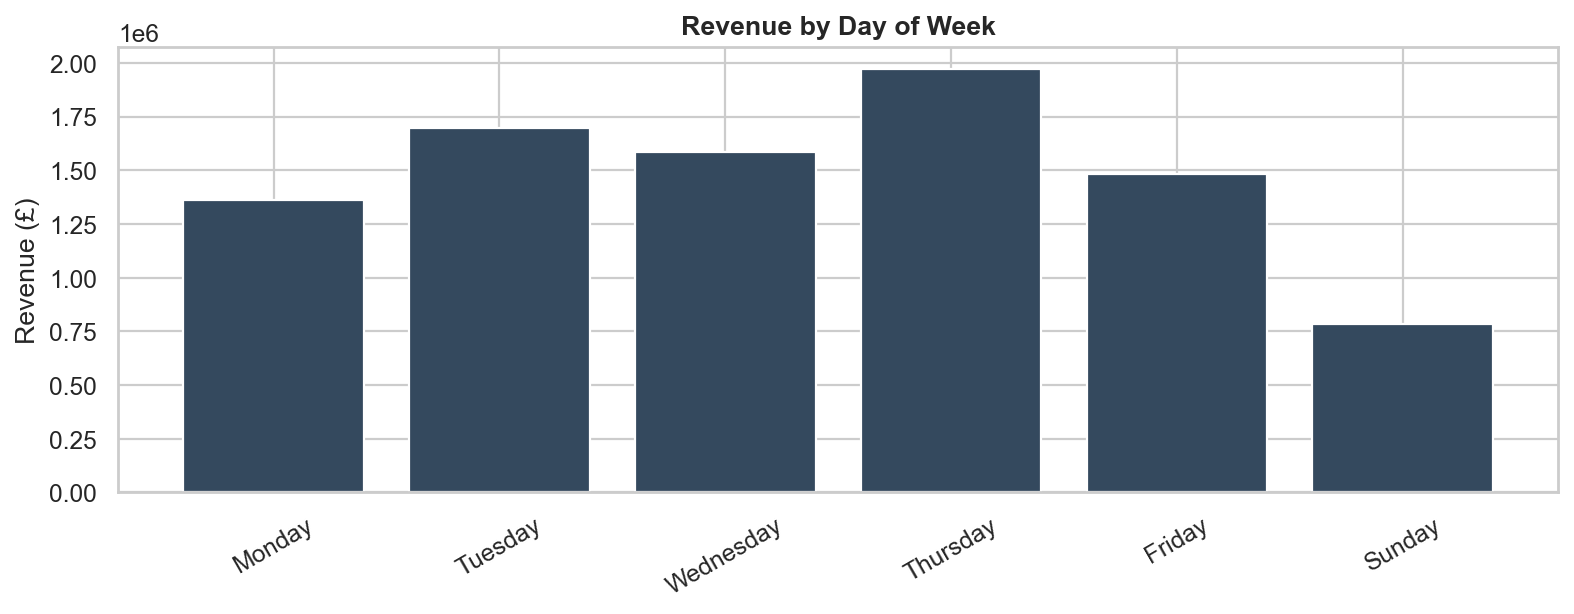
\includegraphics[width=0.85\linewidth]{generated/figures/revenue_by_day.png}}{\fbox{\parbox{0.9\linewidth}{Missing: generated/figures/revenue\_by\_day.png}}}
\caption{Phân bố doanh thu theo ngày trong tuần.}
\end{figure}

\begin{figure}[H]
\centering
\IfFileExists{generated/figures/revenue_by_hour.png}{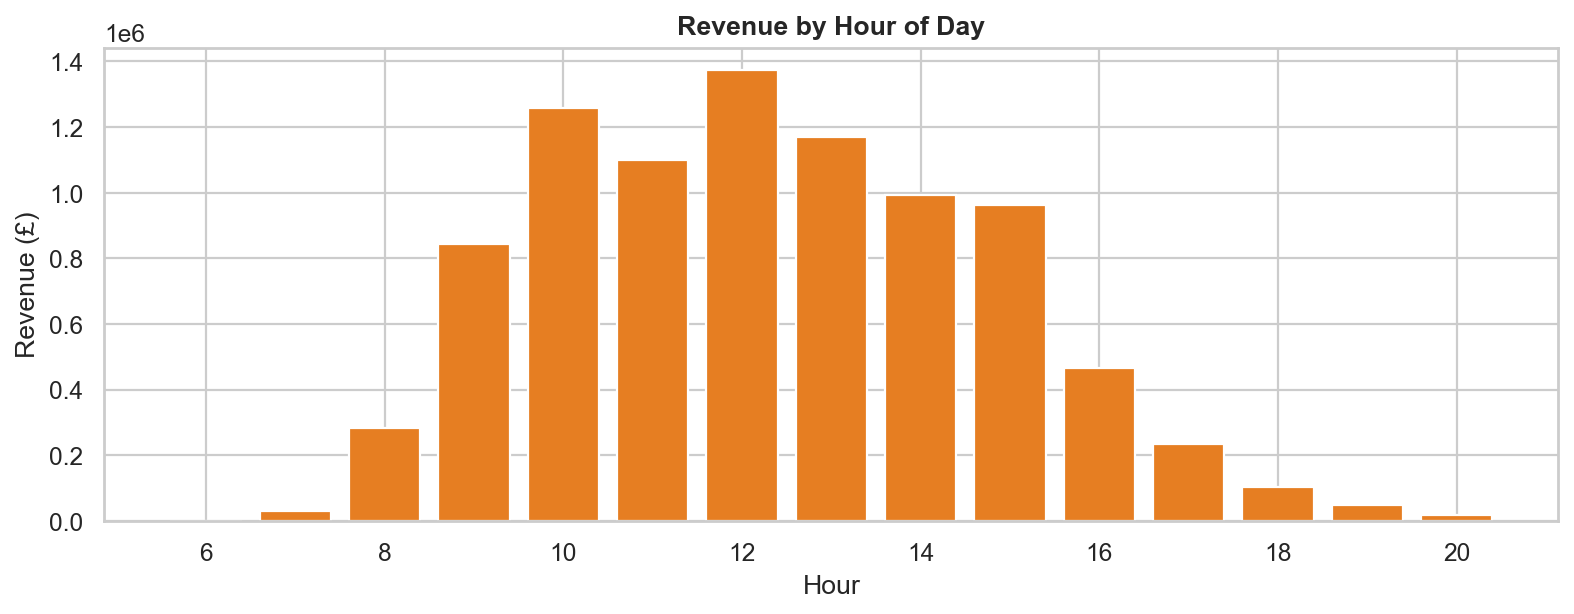
\includegraphics[width=0.85\linewidth]{generated/figures/revenue_by_hour.png}}{\fbox{\parbox{0.9\linewidth}{Missing: generated/figures/revenue\_by\_hour.png}}}
\caption{Phân bố doanh thu theo giờ trong ngày.}
\end{figure}

% =======================================================================
% 6. KNOWLEDGE PRESENTATION / APPLICATION
% =======================================================================
\section{Knowledge Presentation / Application}

\subsection{Interactive Dashboard}
Ứng dụng \texttt{streamlit\_app.py} cung cấp 3 tab chức năng:
\begin{enumerate}
    \item \textbf{Dashboard:} Hiển thị KPI tổng quan (Total Revenue, Total Customers, Average Spend, Average Frequency) cùng với 6+ biểu đồ tương tác Plotly (Monthly Revenue, Top Countries, Top Products, RFM Distribution, Cluster Pie Chart, Cluster Scatter).
    \item \textbf{AI Customer Intelligence:} Nhập CustomerID để xem phân cụm KMeans, dự đoán CLV (XGBoost), và tối đa 5 sản phẩm gợi ý bán chéo (FP-Growth).
    \item \textbf{Pipeline Log:} Xem nhật ký chi tiết của pipeline ETL + Model Training.
\end{enumerate}

\subsection{Decision Support Applications}
Kết quả phát hiện từ dữ liệu hỗ trợ ra quyết định ở 3 cấp độ:

\begin{table}[H]
\centering
\caption{Ứng dụng kết quả khai phá dữ liệu vào quyết định kinh doanh}
\begin{tabular}{|p{3.5cm}|p{4cm}|p{5cm}|}
\hline
\textbf{Mô hình} & \textbf{Tri thức phát hiện} & \textbf{Hành động kinh doanh} \\
\hline
KMeans Clustering & 4 phân khúc khách hàng & Chiến lược marketing phân biệt: khuyến mãi cho ``At Risk'', loyalty program cho ``Champions'' \\
\hline
XGBoost CLV & Dự đoán chi tiêu tương lai & Phân bổ ngân sách marketing: đầu tư nhiều hơn vào khách hàng có CLV cao \\
\hline
FP-Growth Rules & Mẫu mua hàng đồng thời & Gợi ý bán chéo (cross-sell) trên website, email marketing, bundling sản phẩm \\
\hline
\end{tabular}
\end{table}

% =======================================================================
% 7. PIPELINE LOGGING
% =======================================================================
\section{Pipeline Logging and Reproducibility}
Pipeline ghi chi tiết mọi bước vào file \texttt{report/generated/pipeline.log}, bao gồm:
\begin{itemize}
    \item Thời gian thực thi của từng phase (Extract, Transform, Load, Train, Visualize).
    \item Số lượng bản ghi tại mỗi bước làm sạch.
    \item Thống kê mô tả dữ liệu.
    \item Kết quả huấn luyện mô hình (Silhouette, RMSE, R², feature importance).
    \item Cluster profile (RFM trung bình mỗi cụm).
    \item Top 5 association rules.
\end{itemize}

Toàn bộ kết quả được lưu vào \texttt{report/generated/summary.json} dưới dạng JSON có thể tái sử dụng.

\subsection{Generated Artifacts}
Pipeline tạo ra các file sau:
\begin{itemize}
    \item \textbf{Mô hình:} \texttt{output/models/kmeans.pkl}, \texttt{xgb\_model.pkl}, \texttt{rules.pkl}, \texttt{scaler.pkl}
    \item \textbf{Báo cáo:} \texttt{report/generated/summary.json}, \texttt{metrics.tex}, \texttt{pipeline.log}
    \item \textbf{Hình ảnh:} 17 file PNG trong \texttt{report/generated/figures/}
    \item \textbf{Database:} PostgreSQL (hoặc SQLite fallback \texttt{retail\_dw\_fallback.db})
\end{itemize}

% =======================================================================
% 8. CONCLUSION AND FUTURE WORK
% =======================================================================
\section{Conclusion and Future Work}

\subsection{Main Findings and Contributions}
\begin{enumerate}
    \item Xây dựng thành công pipeline ETL tự động end-to-end với khả năng fallback (PostgreSQL → SQLite).
    \item Star Schema cho Data Warehouse bán lẻ với 4 bảng chiều và 1 bảng sự kiện.
    \item KMeans phân cụm 4 phân khúc khách hàng có ý nghĩa kinh doanh rõ ràng.
    \item XGBoost dự đoán CLV với kết quả R² cho thấy mô hình có khả năng giải thích.
    \item FP-Growth sinh luật kết hợp có giá trị cho bán chéo sản phẩm.
    \item Dashboard tương tác kết hợp BI và AI serving.
\end{enumerate}

\subsection{Limitations}
\begin{itemize}
    \item \textbf{Dữ liệu:} Chỉ 1 năm dữ liệu, thiếu thông tin nhân khẩu học khách hàng.
    \item \textbf{Mô hình K-Means:} Giả định cụm hình cầu, có thể không phù hợp nếu phân bố phức tạp. Chưa thử nghiệm DBSCAN hay Gaussian Mixture.
    \item \textbf{XGBoost:} Chưa tối ưu hyperparameter (Grid Search, Bayesian Optimization).
    \item \textbf{FP-Growth:} Chỉ áp dụng cho thị trường UK, chưa mở rộng ra toàn bộ quốc gia.
    \item \textbf{Dashboard:} Chưa có authentication, chưa deploy lên cloud.
\end{itemize}

\subsection{Future Work}
\begin{enumerate}
    \item Tích hợp thêm nguồn dữ liệu (website analytics, customer reviews) vào DW.
    \item Thử nghiệm Deep Learning (LSTM, Transformer) cho time-series CLV prediction.
    \item Deploy pipeline lên cloud (AWS, GCP) với Apache Airflow scheduler.
    \item Áp dụng DBSCAN hoặc Hierarchical Clustering cho phân cụm linh hoạt hơn.
    \item Xây dựng A/B testing framework cho đánh giá hiệu quả recommendation.
    \item Thêm real-time streaming với Apache Kafka cho cập nhật dữ liệu liên tục.
    \item Sử dụng Power BI hoặc Tableau cho enterprise-grade visualization.
\end{enumerate}

\end{document}
